\section{Resultat} % (fold)
\label{sec:resultat}
    \subsection{Algoritm} % (fold)
    \label{sub:algoritm}
        För att möjliggöra automatisk kalibrering av panelens ljussensor har projektet utvecklat en sökalgoritm med positionsregistrering och stegreducering. \bigskip

        Algoritmen söker kontinuerligt stegvis efter det maximala inlästa värdet tills inga kringliggande större värden påträffas och justerar i varje söksteg panelens korrigeringsvärde för ljussensorn, vilket får panelen att vrida sig till den position som ger solljusets fokus i ljussensors korrigerade mittpunkt. Sökning sker i fyra riktningar, representerade av väderstrecksuttryck motsvarande den koordinatsystemsrepresentation panelen har för korrigeringsvärden där positiva x och y är öst respektive nord, och sker medurs med utgångsriktning österut. Om ett lika stort eller större värde avläses efter en vridning av panelen så kommer nästkommande undersökta position vara i samma riktning som den senast utförda, då avlästa värden kan representeras enligt figur~\ref{fig:array}. Algoritmen registrerar besökta positioner så att samma position ej undersöks upprepade gånger. Flödesschema för algoritmen finnes i bilaga \ref{sec:sokalgoritm_flow}. \bigskip

        Tillgången till kontinuerligt solljus är en förutsättning för kalibrering av enheter tagna i bruk då variationer i molnighet markant påverkar ljusintensiteten och således det avlästa värdet. I händelse av längre tids molnighet deaktiveras ljussensorn av panelens mjukvara och kalibrering går då ej att genomföra. Om så sker under pågående kalibrering återställs panelens korrigeringsvärden till de värden som var aktuella innan den automatiska kalibreringen startade. För att ytterligare motverka oförutsedda problem vid kalibreringstillfället har kontroller för timeout och korrigeringsvärdenas rimlighet implementerats, där båda kontrollerna vid utslag avbryter sökningen och korrigeringsvärdena återställs.

    % subsection algoritm (end)
    \subsection{Optisk kommunikation} % (fold)
    \label{sub:optisk_kommunikation}

        Kommunikationen mellan det upplysta rummet och solpanelen på taket kan upprättas med hjälp av två mikrokontroller, en för sändning av data och en för mottagande.\bigskip

        Den lösning som detta projekt presenterar består mikrokonrollerkortet av Arduino Uno revision 3 (för fullständig specifikation se bilaga \ref{sub:arduino_spec})\cite{ardu}. Till sändaren kopplas en lysdiod till det gränssnitt som skickar data via den seriella standarden, vilket då omvandlar från RS-232 standardens höga- och låga läge, till ljus på och ljus av. Till mottagaren kopplas en fotoresistor, en resistor som ändrar motståndet när den träffas av ljus, vilket gör att när den kopplas in till det seriella gränssnittet skapar resistorn spänningsförändringar som registreras som högt eller lågt värde av standarden. \bigskip

        För att möjliggöra överföringen används den i förhållandevis låga överföringshastigheten om 300 baud, vilket gör att komponenterna (fotoresistorn och lysdioden), hinner ändra sina värden under den tid de förväntas göra det på, då dessa komponenter inte är särskilt utformade för denna uppgift och innehåller vissa fördröjningar vid skifte av tillstånd. \bigskip

        Den data som avses skickas i denna kommunikation består av ett 16 bitars värde, det vill säga två byte. Med en överföringshastighet om 300 baud ger det en teoretisk möjlighet att skicka $\frac{300 \,\textit{baud}}{8 \, bit \cdot 2} = 18,75 \, \text{värden per sekund}$. Den faktiska hastigheten blir något lägre då extra bitar skickas enligt RS-232 protokollet, men överföringshastigheten är inte att anses som ett hinder i denna implementation.

        \begin{figure}[h]
        \centering
            \begin{subfigure}[hbt]{0.35\textwidth}
                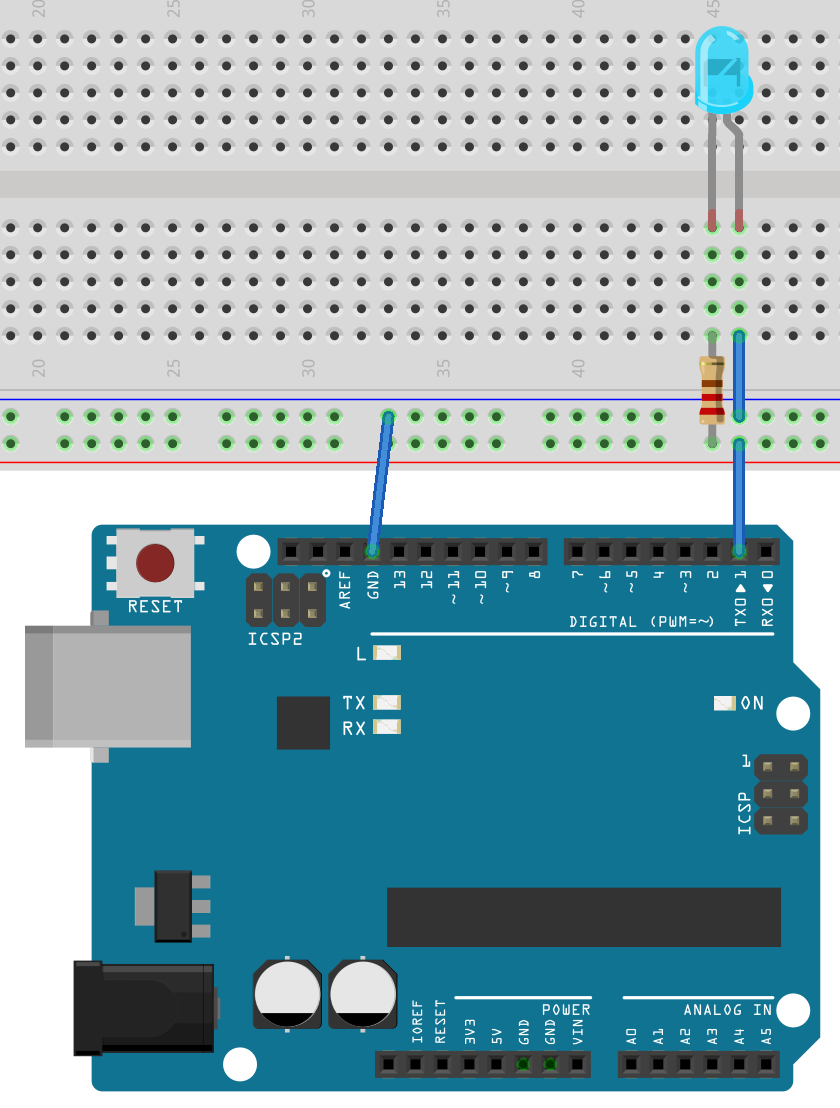
\includegraphics[width=\textwidth]{res/img/led}    
            \end{subfigure}
            \begin{subfigure}[hbt]{0.35\textwidth}
                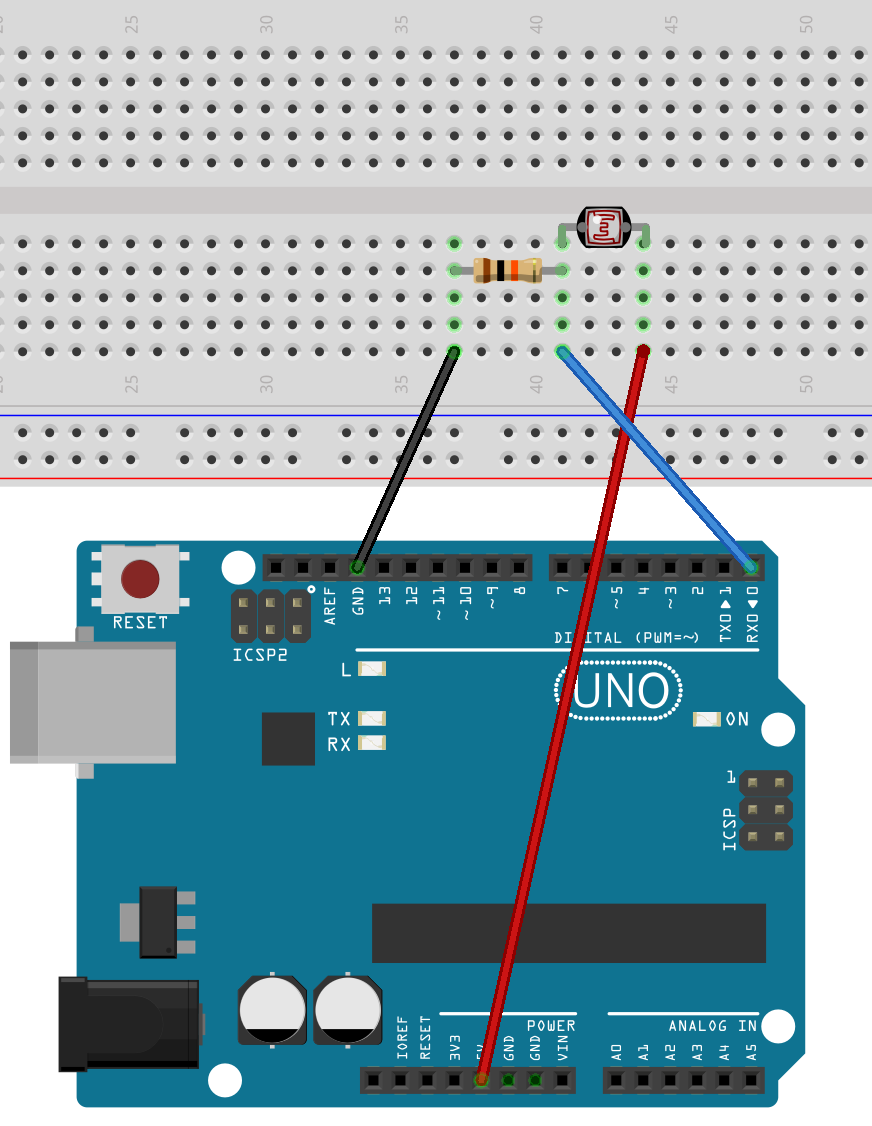
\includegraphics[width=\textwidth]{res/img/resistor}    
            \end{subfigure}
        \caption{Schema över sändare/mottagare}\label{fig:schem}
        \end{figure}


    % subsection optisk_kommunikation (end)
    
% section resultat (end)